\ifthenelse{\equal{\lang}{en}}{
\section{Books Studied (cont.)}

\bookCard
    {\bookCover{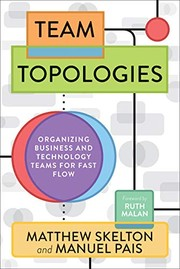
\includegraphics[width=15mm]{img/books/team_topologies.jpg}}}
    {Team Topologies}
    {240p -- Moderate}
    {\fivestars}
    {M. Skelton \& M. Pais}
    {02/2026}
    {Software architecture and team organization co-evolve (Conway's Law), so fast flow requires four clear team types with well-defined interaction modes.}
    {I loved this book. While trying to expand my soft-skills set, I came across this book that closes the gap between teams and code. For example, something that blew my mind is that how a company is organized determines how you organize the code (the folder structure). I learned there are different ways to isolate code by team: strong isolation (separate repositories), weak isolation (each person works in a separate folder within the same repo), or no isolation (members of the same team work on the same files). It then covers 4 fundamental team topologies (continuous business value generation, enabling teams, etc.) and how they communicate or interrelate. A brilliant book.}

\bookCard
    {\bookCover{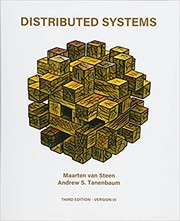
\includegraphics[width=15mm]{img/books/distributed_systems.jpg}}}
    {Distributed Systems}
    {640p -- Very Hard}
    {\twostars}
    {A. Tanenbaum \& M. van Steen}
    {01/2026}
    {A distributed system must appear as one coherent, resource-sharing, scalable system despite being built from independent, failure-prone nodes across a network.}
    {A super dense, heavy read. Still, I put in the full effort to finish it, since I needed that exposure to distributed systems networking. It made me realize distributed systems don't have infinite forms -- on the contrary, every topology is well studied. It sometimes starts from a very specific problem, like "how do you sync a clock across 100 computers? which clock do you use? how do you know which piece of data came before another?". This kind of book is a grind to study, but these are structures that show up now and then in software development, and knowing them gives you the confidence that you're building things right. A very theoretical book.}

\bookCard
    {\bookCover{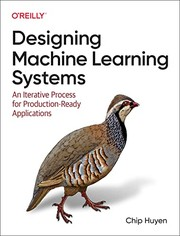
\includegraphics[width=15mm]{img/books/designing_ml.jpg}}}
    {Designing Machine Learning Systems}
    {386p -- Hard}
    {\fourstars}
    {Chip Huyen}
    {10/2025}
    {Data quality (sampling, labeling, class imbalance, augmentation) is as critical as modeling, since biased or imbalanced training data drives poor real-world predictions.}
    {A very enjoyable read -- I remember thinking it was spectacular. It introduced me to "data drift" and the most common data problems. That said, I can't say it blew my mind: it overlaps quite a bit with knowledge I already had... but even so, I must have learned something new, even though I can't recall exactly what right now. Even so, I loved reading it, and its follow-up, AI Engineering, that one I found fabulous.}
}{
\section{Libros Estudiados (cont.)}

\bookCard
    {\bookCover{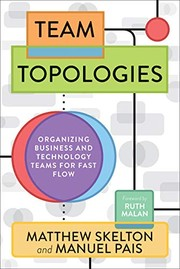
\includegraphics[width=15mm]{img/books/team_topologies.jpg}}}
    {Team Topologies}
    {240p -- Moderado}
    {\fivestars}
    {M. Skelton y M. Pais}
    {02/2026}
    {La arquitectura de software y la organización de equipos co-evolucionan (Ley de Conway), por lo que un flujo rápido requiere cuatro tipos de equipo bien definidos.}
    {Me encantó este libro. Intentando expandir mi set de habilidades blandas, me topé con este libro que cierra el gap entre equipos y código. Por ejemplo, algo que me voló la cabeza es que cómo está organizada la empresa determina cómo uno organiza el código (la estructura de carpetas). Aprendí que existen diferentes formas de aislar el código por equipos: aislación fuerte (repositorios separados), aislación débil (cada individuo trabaja en una carpeta separada del mismo repo), o sin aislación (integrantes del mismo team trabajan con los mismos archivos). Luego habla de 4 estructuras fundamentales de equipos (generación de valor de negocio continuo, facilitadores, etc.) y cómo se comunican o interrelacionan entre sí. Es un libro brillante.}

\bookCard
    {\bookCover{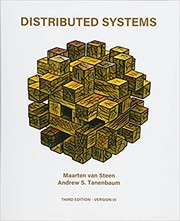
\includegraphics[width=15mm]{img/books/distributed_systems.jpg}}}
    {Distributed Systems}
    {640p -- Muy Difícil}
    {\twostars}
    {A. Tanenbaum y M. van Steen}
    {01/2026}
    {Un sistema distribuido debe presentarse como un único sistema coherente y escalable, a pesar de estar construido con nodos independientes y propensos a fallar.}
    {Es un libro súper denso y pesado de leer. Sin embargo hice el esfuerzo completo de terminarlo, pues necesitaba esa exposición a sistemas distribuidos en red. Me hizo ver que los sistemas distribuidos no tienen infinitas formas -- al contrario, cada topología está bien estudiada. A veces arranca con un problema muy particular, como "¿cómo sincronizar un clock entre 100 computadoras? ¿qué reloj usamos? ¿cómo saber qué dato vino antes que cuál?". Este tipo de libro es sacrificado de estudiar, pero son estructuras que cada tanto aparecen en el desarrollo de software, y saberlas te da la confianza de que estás desarrollando las cosas bien. Es un libro muy teórico.}

\bookCard
    {\bookCover{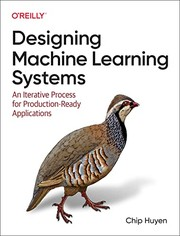
\includegraphics[width=15mm]{img/books/designing_ml.jpg}}}
    {Designing Machine Learning Systems}
    {386p -- Difícil}
    {\fourstars}
    {Chip Huyen}
    {10/2025}
    {La calidad de los datos (muestreo, etiquetado, desbalance de clases, aumentación) es tan crítica como el modelado: datos sesgados o desbalanceados generan malas predicciones en producción.}
    {Es un libro muy ameno de leer -- recuerdo que al leerlo me pareció espectacular. Me introdujo en "data drift" y en los problemas de datos más comunes. Sin embargo no puedo decir que "me voló la cabeza": es un libro que se solapa bastante con otros conocimientos que ya tenía... pero aún así, algo nuevo habré aprendido, aunque ahora mismo no recuerde exactamente qué. Aun así me encantó haberlo leído, y su continuación, AI Engineering, ese sí me pareció fabuloso.}
}
